% Depression Speech Detection - Dissertation Presentation
% Author: Nile
% University of Glasgow, Level 4 Computer Science
% February 2026

\documentclass[aspectratio=169,11pt]{beamer}

% ============================================
% Theme and Color Setup
% ============================================
\usetheme{Madrid}
\usecolortheme{seahorse}

% Custom colors - professional blue/grey palette
\definecolor{uofgblue}{RGB}{0,78,124}
\definecolor{accentblue}{RGB}{0,119,182}
\definecolor{lightgrey}{RGB}{248,249,250}
\definecolor{darkgrey}{RGB}{73,80,87}
\definecolor{successgreen}{RGB}{25,135,84}
\definecolor{warningorange}{RGB}{255,193,7}

\setbeamercolor{palette primary}{bg=uofgblue,fg=white}
\setbeamercolor{palette secondary}{bg=accentblue,fg=white}
\setbeamercolor{structure}{fg=uofgblue}
\setbeamercolor{title}{fg=uofgblue}
\setbeamercolor{frametitle}{fg=uofgblue,bg=lightgrey}
\setbeamercolor{block title}{bg=uofgblue,fg=white}
\setbeamercolor{block body}{bg=lightgrey,fg=darkgrey}
\setbeamercolor{alerted text}{fg=accentblue}

% Remove navigation symbols
\setbeamertemplate{navigation symbols}{}

% Add slide numbers
\setbeamertemplate{footline}{
    \hfill\insertframenumber/\inserttotalframenumber\hspace{2em}\vspace{1em}
}

% ============================================
% Packages
% ============================================
\usepackage{graphicx}
\usepackage{booktabs}
\usepackage{fontawesome5}
\usepackage{tikz}
\usetikzlibrary{shapes,arrows,positioning,calc}
\usepackage{xcolor}
\usepackage{multicol}

% Figure path
\graphicspath{{../figures/advanced/}}

% ============================================
% Title Information
% ============================================
\title[Depression \& Speech]{\Large Identifying Depression Through Speech}
\subtitle{A Comparative Analysis of Acoustic Features\\in Read and Spontaneous Speech}
\author{Nile}
\institute{University of Glasgow\\School of Computing Science}
\date{Level 4 Dissertation \\ February 2026}

% ============================================
% Document
% ============================================
\begin{document}

% --------------------------------------------
% SLIDE 1: Title
% --------------------------------------------
\begin{frame}[plain]
    \vfill
    \centering
    
    {\LARGE\bfseries\color{uofgblue} Identifying Depression Through Speech}
    
    \vspace{0.5cm}
    
    {\large\color{darkgrey} A Comparative Analysis of Acoustic Features\\in Read and Spontaneous Speech}
    
    \vspace{1cm}
    
    \textbf{Nile}
    
    \vspace{0.3cm}
    
    {\small University of Glasgow\\School of Computing Science\\Level 4 Dissertation}
    
    \vspace{0.8cm}
    
    {\footnotesize February 2026}
    
    \vfill
\end{frame}

% --------------------------------------------
% SLIDE 2: Why This Matters
% --------------------------------------------
\begin{frame}{Why This Matters}
    \begin{columns}[T]
        \begin{column}{0.48\textwidth}
            \textbf{\color{uofgblue}\faExclamationTriangle\hspace{0.3em} The Problem}
            
            \vspace{0.3cm}
            
            \begin{itemize}
                \item \textbf{280+ million} affected globally
                \item \textbf{1 in 6} UK adults weekly
                \item Diagnosis relies on self-report
                \item Inter-rater reliability as low as \textbf{0.28 kappa}
                \item Access barriers to specialist care
            \end{itemize}
        \end{column}
        
        \begin{column}{0.48\textwidth}
            \textbf{\color{successgreen}\faLightbulb\hspace{0.3em} The Opportunity}
            
            \vspace{0.3cm}
            
            \begin{center}
            \begin{tikzpicture}
                \node[draw=accentblue,fill=lightgrey,rounded corners,
                      text width=5cm,align=center,inner sep=12pt] {
                    \faVolumeUp\hspace{0.5em}\textbf{Speech}\\[0.3cm]
                    \small Non-invasive\\
                    \small Remote collection\\
                    \small No specialist equipment
                };
            \end{tikzpicture}
            \end{center}
        \end{column}
    \end{columns}
\end{frame}

% --------------------------------------------
% SLIDE 3: Research Gap
% --------------------------------------------
\begin{frame}{The Research Gap}
    \begin{columns}[T]
        \begin{column}{0.45\textwidth}
            \textbf{\color{darkgrey}\faCheckCircle\hspace{0.3em} What exists}
            
            \vspace{0.3cm}
            
            Deep learning models\\achieving 80\%+ accuracy
            
            \vspace{0.5cm}
            
            \begin{center}
            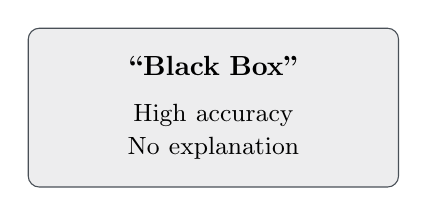
\begin{tikzpicture}
                \node[draw=darkgrey,fill=darkgrey!10,rounded corners,
                      text width=4cm,align=center,inner sep=10pt] {
                    \textbf{``Black Box''}\\[0.2cm]
                    \small High accuracy\\
                    \small No explanation
                };
            \end{tikzpicture}
            \end{center}
        \end{column}
        
        \begin{column}{0.52\textwidth}
            \textbf{\color{accentblue}\faQuestionCircle\hspace{0.3em} What's missing}
            
            \vspace{0.3cm}
            
            \begin{itemize}
                \item \textit{Which} features indicate depression?
                \item Does speech \textit{task type} matter?
            \end{itemize}
            
            \vspace{0.5cm}
            
            \begin{block}{Research Question}
                \small Which acoustic features are most predictive of depression, and how do they differ between \textbf{read} and \textbf{spontaneous} speech?
            \end{block}
        \end{column}
    \end{columns}
\end{frame}

% --------------------------------------------
% SLIDE 4: Approach Overview
% --------------------------------------------
\begin{frame}{Approach Overview}
    \begin{center}
    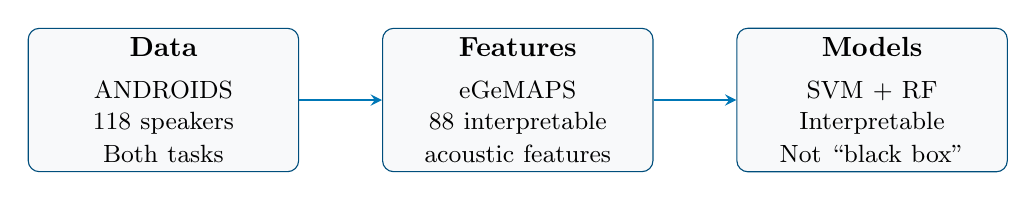
\begin{tikzpicture}[
        box/.style={draw=uofgblue,fill=lightgrey,rounded corners,
                    minimum height=1.5cm,text width=3.2cm,align=center},
        arrow/.style={->,>=stealth,thick,color=accentblue}
    ]
        % Nodes
        \node[box] (data) at (0,0) {\textbf{Data}\\[0.15cm]\small ANDROIDS\\118 speakers\\Both tasks};
        \node[box] (features) at (4.5,0) {\textbf{Features}\\[0.15cm]\small eGeMAPS\\88 interpretable\\acoustic features};
        \node[box] (models) at (9,0) {\textbf{Models}\\[0.15cm]\small SVM + RF\\Interpretable\\Not ``black box''};
        
        % Arrows
        \draw[arrow] (data) -- (features);
        \draw[arrow] (features) -- (models);
    \end{tikzpicture}
    \end{center}
    
    \vspace{0.5cm}
    
    \begin{columns}[T]
        \begin{column}{0.32\textwidth}
            \centering
            \small\color{darkgrey}
            \faUsers\hspace{0.3em} Clinical diagnoses\\
            Same participants\\do both tasks
        \end{column}
        \begin{column}{0.32\textwidth}
            \centering
            \small\color{darkgrey}
            \faMusic\hspace{0.3em} Prosody, spectral\\
            voice quality, timing\\
            Each feature = meaning
        \end{column}
        \begin{column}{0.32\textwidth}
            \centering
            \small\color{darkgrey}
            \faSearch\hspace{0.3em} Deliberately\\
            interpretable\\
            Not deep learning
        \end{column}
    \end{columns}
\end{frame}

% --------------------------------------------
% SLIDE 5: Headline Result
% --------------------------------------------
\begin{frame}{The Headline Result}
    \begin{center}
        {\Large\bfseries\color{uofgblue} Interview speech significantly outperforms reading}
    \end{center}
    
    \vspace{0.3cm}
    
    \begin{columns}
        \begin{column}{0.55\textwidth}
            \centering
            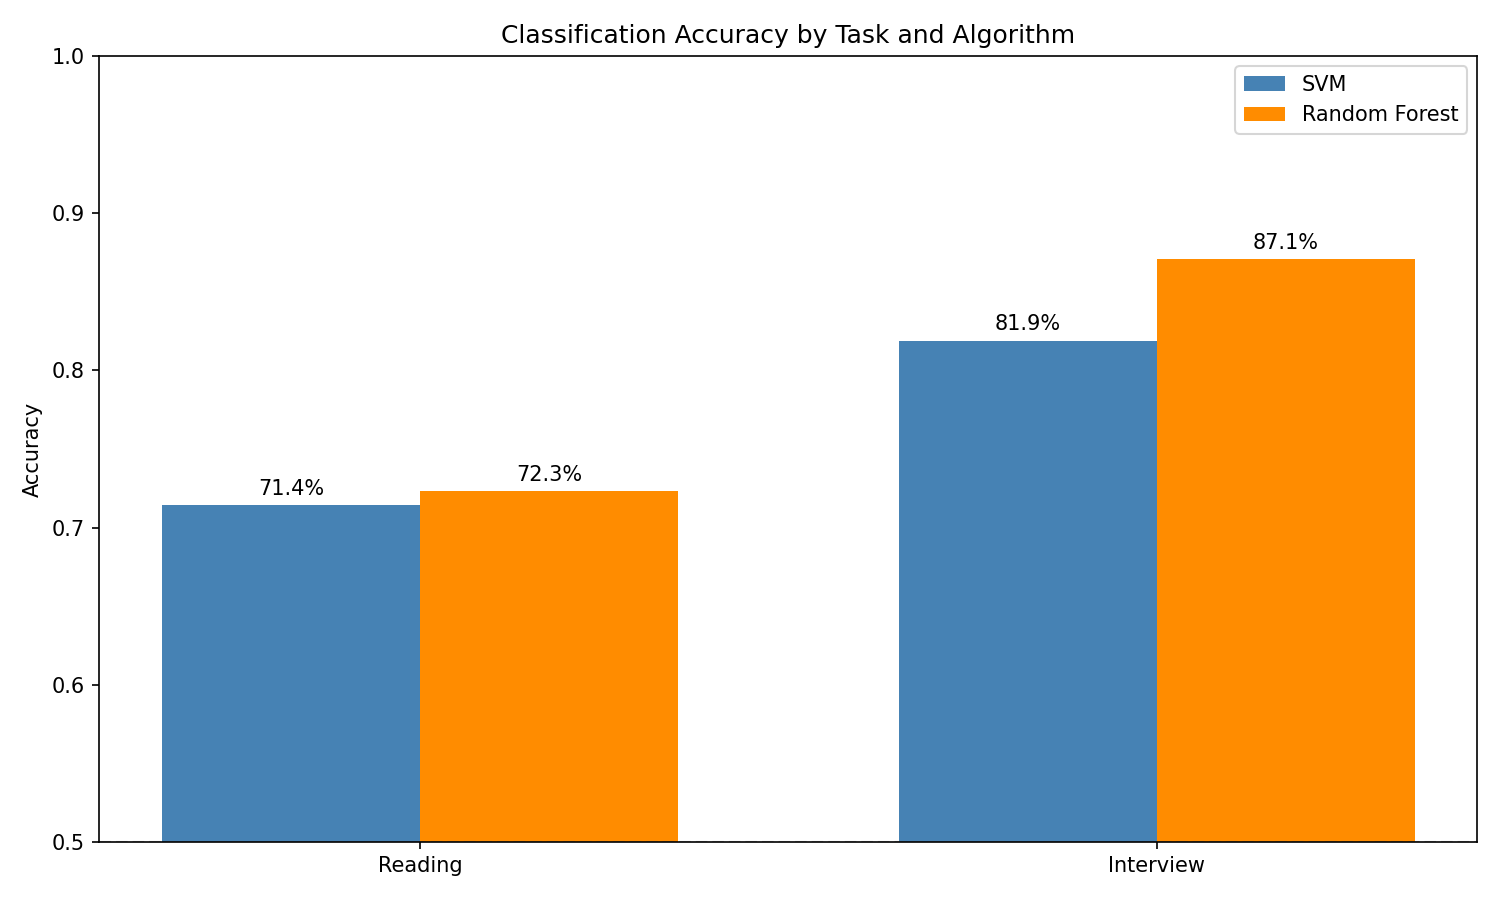
\includegraphics[width=\textwidth]{accuracy_comparison.png}
        \end{column}
        
        \begin{column}{0.42\textwidth}
            \begin{table}
                \centering
                \begin{tabular}{lc}
                    \toprule
                    \textbf{Task} & \textbf{Accuracy} \\
                    \midrule
                    Reading & 72.3\% \\
                    \textbf{Interview} & \textbf{87.1\%} \\
                    \bottomrule
                \end{tabular}
            \end{table}
            
            \vspace{0.5cm}
            
            \begin{itemize}
                \item[\color{successgreen}\faArrowUp] \textbf{+15 points} difference
                \item[\color{accentblue}\faChartLine] p = 0.0055 significant
                \item[\color{successgreen}\faTrophy] Beats prior DL (81.6\%)
            \end{itemize}
        \end{column}
    \end{columns}
\end{frame}

% --------------------------------------------
% SLIDE 6: Feature Divergence
% --------------------------------------------
\begin{frame}{But Here's What's Interesting...}
    \begin{center}
        {\large\bfseries\color{uofgblue} Different features predict depression in each task}
    \end{center}
    
    \vspace{0.3cm}
    
    \begin{columns}[T]
        \begin{column}{0.48\textwidth}
            \begin{block}{\centering Reading Task}
                \centering
                \small
                Spectral slopes\\
                MFCCs\\[0.2cm]
                \textit{Static properties}
            \end{block}
        \end{column}
        
        \begin{column}{0.48\textwidth}
            \begin{block}{\centering Interview Task}
                \centering
                \small
                Variability measures\\
                Temporal dynamics\\[0.2cm]
                \textit{Dynamic properties}
            \end{block}
        \end{column}
    \end{columns}
    
    \vspace{0.5cm}
    
    \begin{center}
        \begin{tikzpicture}
            \node[draw=warningorange,fill=warningorange!15,rounded corners,
                  text width=10cm,align=center,inner sep=15pt] {
                \faExclamationCircle\hspace{0.5em}
                Of top 10 features: \textbf{Only 1 overlaps}\\[0.2cm]
                \small This isn't just ``interview is better'' --- they capture \textbf{qualitatively different information}
            };
        \end{tikzpicture}
    \end{center}
\end{frame}

% --------------------------------------------
% SLIDE 7: Variability Finding
% --------------------------------------------
\begin{frame}{The Variability Finding}
    \begin{columns}
        \begin{column}{0.55\textwidth}
            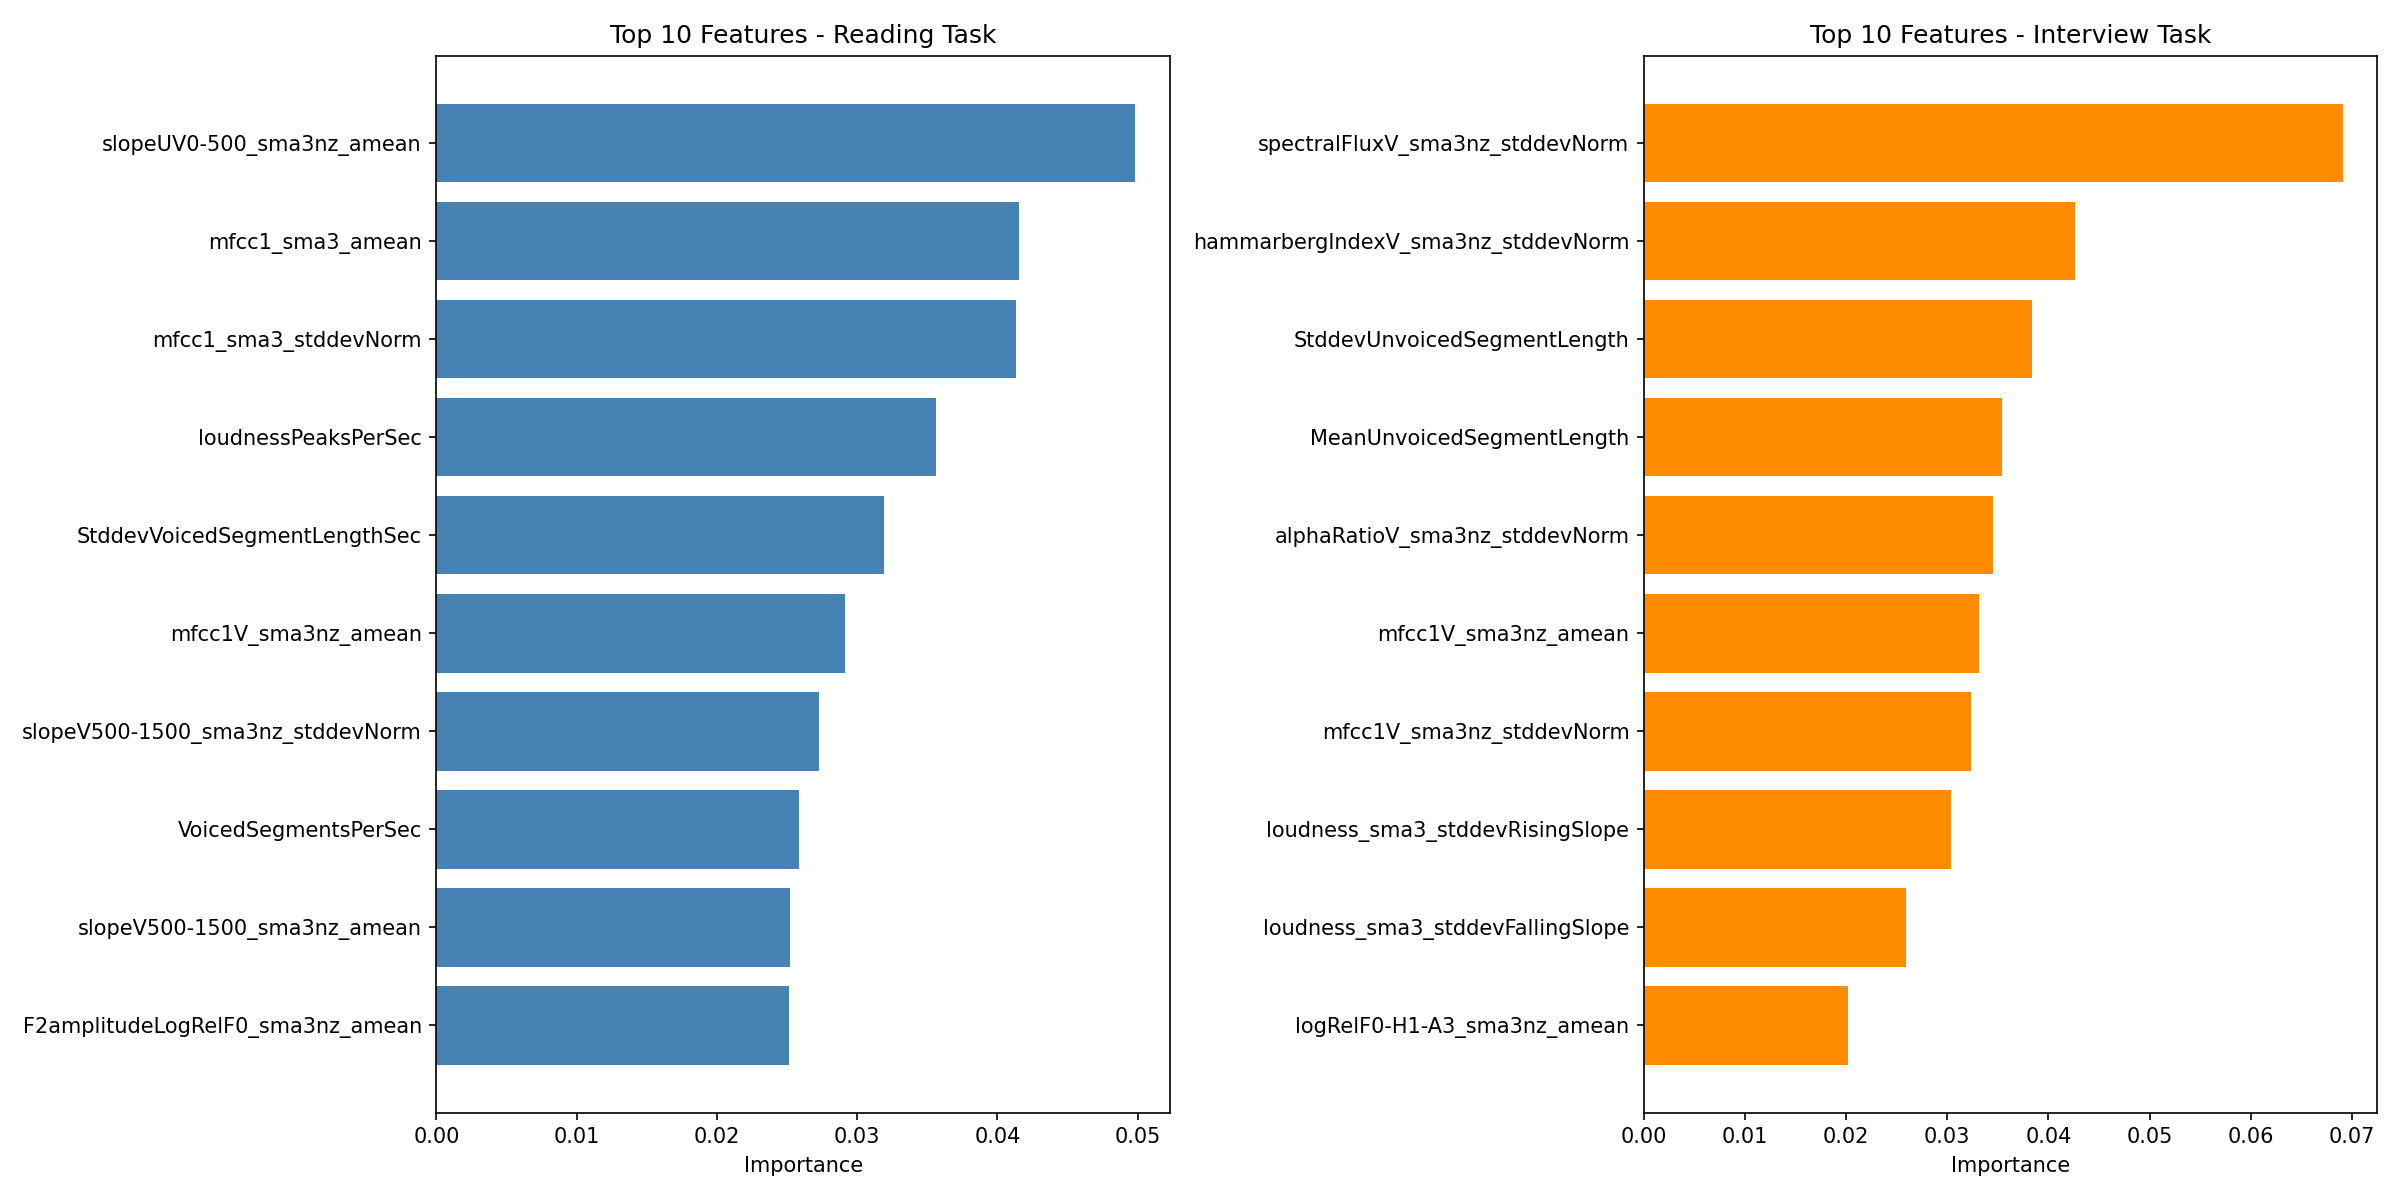
\includegraphics[width=\textwidth]{feature_importance_comparison.png}
        \end{column}
        
        \begin{column}{0.42\textwidth}
            \textbf{\color{uofgblue} Interview: 7/10 are variability}
            
            \vspace{0.3cm}
            
            \small
            \begin{enumerate}
                \item Spectral flux \textit{variability}
                \item Hammarberg index \textit{variability}
                \item Pause duration \textit{variability}
            \end{enumerate}
            
            \vspace{0.4cm}
            
            \textbf{\color{darkgrey} Reading: Only 2/10}
            
            \vspace{0.5cm}
            
            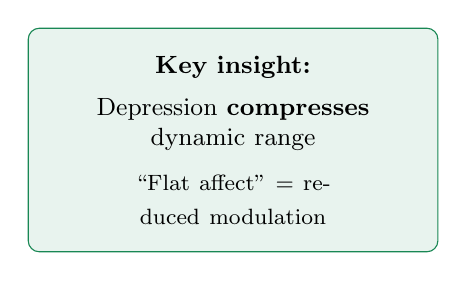
\begin{tikzpicture}
                \node[draw=successgreen,fill=successgreen!10,rounded corners,
                      text width=4.5cm,align=center,inner sep=10pt] {
                    \small\textbf{Key insight:}\\[0.15cm]
                    Depression \textbf{compresses}\\dynamic range\\[0.15cm]
                    \footnotesize ``Flat affect'' = reduced modulation
                };
            \end{tikzpicture}
        \end{column}
    \end{columns}
\end{frame}

% --------------------------------------------
% SLIDE 8: Why Interview Works Better
% --------------------------------------------
\begin{frame}{Why Interview Works Better}
    \begin{center}
        {\large\bfseries\color{uofgblue} Three mechanisms from clinical literature}
    \end{center}
    
    \vspace{0.3cm}
    
    \begin{columns}[T]
        \begin{column}{0.31\textwidth}
            \begin{center}
                {\Large\color{accentblue}\faBrain}
                
                \vspace{0.2cm}
                
                \textbf{Cognitive Load}
            \end{center}
            
            \vspace{0.2cm}
            
            \small
            Spontaneous speech requires planning, retrieval, monitoring
            
            \vspace{0.2cm}
            
            \footnotesize\color{darkgrey}
            Depression impairs executive function $\rightarrow$ pauses, hesitations
        \end{column}
        
        \begin{column}{0.31\textwidth}
            \begin{center}
                {\Large\color{accentblue}\faHeart}
                
                \vspace{0.2cm}
                
                \textbf{Emotional Engagement}
            \end{center}
            
            \vspace{0.2cm}
            
            \small
            Interview topics engage affect (mood, relationships)
            
            \vspace{0.2cm}
            
            \footnotesize\color{darkgrey}
            Depression alters expression $\rightarrow$ only visible when emotions relevant
        \end{column}
        
        \begin{column}{0.31\textwidth}
            \begin{center}
                {\Large\color{accentblue}\faWaveSquare}
                
                \vspace{0.2cm}
                
                \textbf{Prosodic Freedom}
            \end{center}
            
            \vspace{0.2cm}
            
            \small
            Reading follows punctuation; conversation allows natural modulation
            
            \vspace{0.2cm}
            
            \footnotesize\color{darkgrey}
            Depression compresses this natural range
        \end{column}
    \end{columns}
    
    \vspace{0.5cm}
    
    \begin{center}
        \color{darkgrey}\small
        Interview captures all three channels. Reading suppresses them.
    \end{center}
\end{frame}

% --------------------------------------------
% SLIDE 9: Implications
% --------------------------------------------
\begin{frame}{Implications}
    \begin{columns}[T]
        \begin{column}{0.31\textwidth}
            \textbf{\color{uofgblue}\faStethoscope\hspace{0.3em} Clinical Practice}
            
            \vspace{0.3cm}
            
            \small
            \begin{itemize}
                \item Task selection $>$ algorithm choice
                \item Spontaneous $>$ reading for screening
                \item Measure \textbf{variability}, not just means
            \end{itemize}
        \end{column}
        
        \begin{column}{0.31\textwidth}
            \textbf{\color{uofgblue}\faFlask\hspace{0.3em} Research}
            
            \vspace{0.3cm}
            
            \small
            \begin{itemize}
                \item Single-task studies miss markers
                \item Feature importance is task-contingent
                \item ``MFCCs are best'' may only hold for reading
            \end{itemize}
        \end{column}
        
        \begin{column}{0.31\textwidth}
            \textbf{\color{uofgblue}\faCogs\hspace{0.3em} System Design}
            
            \vspace{0.3cm}
            
            \small
            \begin{itemize}
                \item Elicit spontaneous speech
                \item Use open-ended questions
                \item Prioritise temporal dynamics
            \end{itemize}
        \end{column}
    \end{columns}
\end{frame}

% --------------------------------------------
% SLIDE 10: Limitations
% --------------------------------------------
\begin{frame}{Limitations}
    \begin{columns}[T]
        \begin{column}{0.48\textwidth}
            \textbf{\color{warningorange}\faExclamationTriangle\hspace{0.3em} Most Serious}
            
            \vspace{0.3cm}
            
            \begin{itemize}
                \item \textbf{Italian speech only}\\
                      \small\color{darkgrey} Features may not transfer to English
                      
                \vspace{0.2cm}
                      
                \item \normalsize\color{black}\textbf{Modest sample size}\\
                      \small\color{darkgrey} 118 speakers
            \end{itemize}
        \end{column}
        
        \begin{column}{0.48\textwidth}
            \textbf{\color{darkgrey}\faInfoCircle\hspace{0.3em} Moderate}
            
            \vspace{0.3cm}
            
            \begin{itemize}
                \item Binary labels only\\
                      \small\color{darkgrey} No severity information
                      
                \vspace{0.2cm}
                      
                \item \normalsize\color{black}Gender imbalance (72\% female)\\
                      \small\color{darkgrey} Women misclassified slightly more
            \end{itemize}
        \end{column}
    \end{columns}
    
    \vspace{0.7cm}
    
    \begin{center}
        
\begin{tikzpicture}
            \node[draw=accentblue,fill=accentblue!10,rounded corners,
                  text width=10cm,align=center,inner sep=12pt] {
                \faArrowRight\hspace{0.5em}
                \textbf{Cross-corpus validation essential} before clinical deployment
            };
        \end{tikzpicture}
    \end{center}
\end{frame}

% --------------------------------------------
% SLIDE 11: Conclusion
% --------------------------------------------
\begin{frame}{Conclusion}
    \begin{center}
        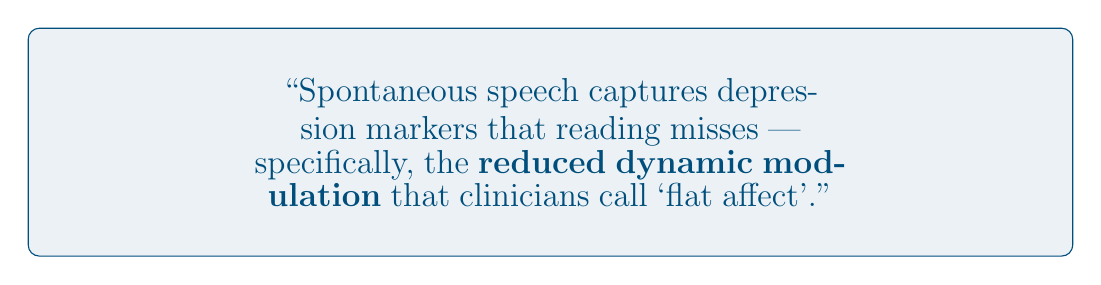
\begin{tikzpicture}
            \node[draw=uofgblue,fill=uofgblue!8,rounded corners,
                  text width=12cm,align=center,inner sep=18pt] {
                \large\color{uofgblue}
                ``Spontaneous speech captures depression markers that reading misses ---\\
                specifically, the \textbf{reduced dynamic modulation} that clinicians call `flat affect'.''
            };
        \end{tikzpicture}
    \end{center}
    
    \vspace{0.5cm}
    
    \textbf{\color{uofgblue} Contributions:}
    
    \vspace{0.2cm}
    
    \begin{columns}[T]
        \begin{column}{0.48\textwidth}
            \begin{enumerate}
                \item Quantified the task effect\\
                      \small\color{darkgrey} +15 points, p = 0.0055
                      
                \vspace{0.15cm}
                      
                \item \normalsize\color{black}Showed features are task-specific\\
                      \small\color{darkgrey} Only 1/10 overlap
            \end{enumerate}
        \end{column}
        
        \begin{column}{0.48\textwidth}
            \begin{enumerate}
                \setcounter{enumi}{2}
                \item Interpretable methods match DL\\
                      \small\color{darkgrey} 87.1\% vs 81.6\% prior work
                      
                \vspace{0.15cm}
                      
                \item \normalsize\color{black}Identified key signal: \textbf{variability}\\
                      \small\color{darkgrey} 7/10 top interview features
            \end{enumerate}
        \end{column}
    \end{columns}
\end{frame}

% --------------------------------------------
% SLIDE 12: Questions
% --------------------------------------------
\begin{frame}{Questions?}
    \vfill
    
    \begin{center}
        {\Huge\color{accentblue}\faComments}
        
        \vspace{0.8cm}
        
        {\Large\bfseries\color{uofgblue} Thank you}
        
        \vspace{0.5cm}
        
        {\large Nile}\\
        {\small University of Glasgow}
    \end{center}
    
    \vfill
    
    \begin{center}
        \footnotesize\color{darkgrey}
        \begin{tabular}{rl}
            \textbf{Key numbers:} & 87.1\% interview vs 72.3\% reading (p = 0.0055) \\
            & 1/10 feature overlap • 7/10 interview features are variability \\
        \end{tabular}
    \end{center}
    
    \vfill
\end{frame}

\end{document}
